\documentclass[17pt, t, lualatex]{beamer}

\title{Between Two Worlds\\\large Surrogate Gradients for Gradient-Based Parameter Estimation in Simplified Neuron Models}
\date{January 12th, 2026}
\institute[KTH]{KTH Royal Institute of Technology}
\author{Paul Mayer}

\usepackage{amsmath,amssymb,mathtools}
\usepackage{multicol}
\usepackage{hyperref}
\usepackage{booktabs}
\usepackage{tikz}
\usetikzlibrary{shapes,arrows,positioning,calc,decorations.pathreplacing}

% Probably load as late as possible
\usetheme[engine=lualatex, mathshape=sf, fontdir=kthpq-files/fonts/Figtree/]{kthpq}
\setmonofont{Bitstream Vera Sans Mono}[Scale=.9]

\begin{document}

\inserttitlepage

%% ============================================================
%% SLIDE 2: Motivation
%% ============================================================
\begin{frame}{Motivation: Large-Scale Brain Simulation}
\begin{center}
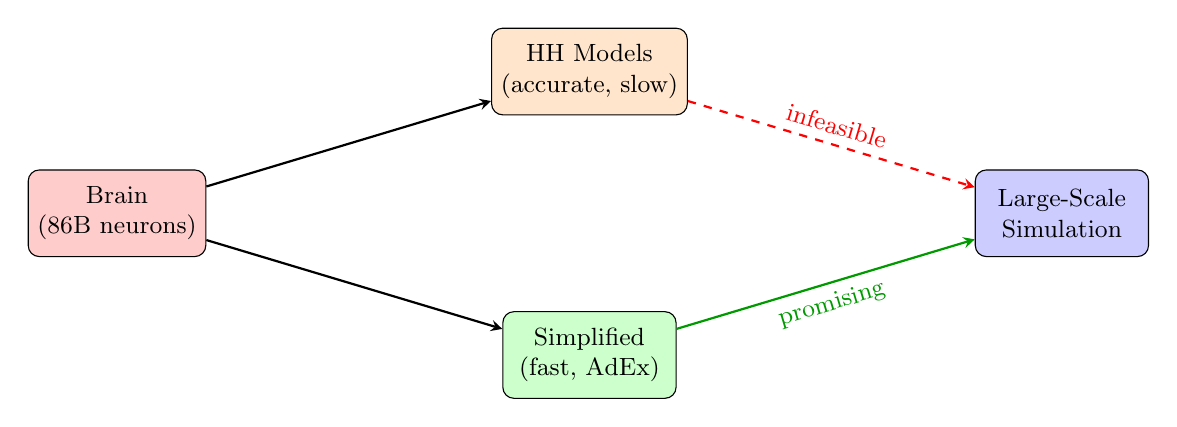
\begin{tikzpicture}[
    box/.style={draw, rounded corners, minimum width=2.2cm, minimum height=1.1cm, align=center, font=\small},
    arrow/.style={->, thick, >=stealth}
]
    \node[box, fill=red!20] (brain) at (0,0) {Brain\\(86B neurons)};
    \node[box, fill=orange!20] (hh) at (6,1.8) {HH Models\\(accurate, slow)};
    \node[box, fill=green!20] (simple) at (6,-1.8) {Simplified\\(fast, AdEx)};
    \node[box, fill=blue!20] (sim) at (12,0) {Large-Scale\\Simulation};

    \draw[arrow] (brain) -- (hh);
    \draw[arrow] (brain) -- (simple);
    \draw[arrow, dashed, red] (hh) -- node[above, sloped, font=\small] {infeasible} (sim);
    \draw[arrow, green!60!black] (simple) -- node[below, sloped, font=\small] {promising} (sim);
\end{tikzpicture}
\end{center}

\vspace{0.5cm}
\textbf{Problem:} Simplified models need parameter fitting, but are \alert{non-differentiable}
\end{frame}

%% ============================================================
%% SLIDE 3: AdEx Model
%% ============================================================
\begin{frame}{The AdEx Model}
\textbf{Membrane potential:}
\begin{equation}
  C \frac{dV}{dt} = -g_L(V - E_L) + g_L\Delta_T e^{\frac{V-V_T}{\Delta_T}} + I - w
  \label{eq:membrane-potential}
\end{equation}

\textbf{Adaptation current:}
\begin{equation}
  \tau_w \frac{dw}{dt} = a(V - E_L) - w
  \label{eq:adaption-current}
\end{equation}
\textbf{Reset condition:}
\begin{equation}
  \text{if } V > V_{\text{th}}: \begin{cases} V \rightarrow V_r \\ w \rightarrow w + b \end{cases}
  \label{eq:reset}
\end{equation}
\end{frame}

%% ============================================================
%% SLIDE 4: The Problem
%% ============================================================
\begin{frame}{The Differentiability Problem}
\begin{center}
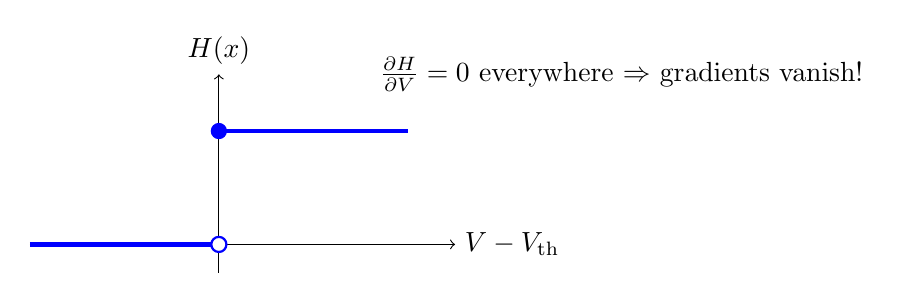
\begin{tikzpicture}[scale=1.2]
    % Heaviside function
    \draw[->] (-2,0) -- (2.5,0) node[right] {$V - V_{\text{th}}$};
    \draw[->] (0,-0.3) -- (0,1.8) node[above] {$H(x)$};

    % Step function
    \draw[blue, ultra thick] (-2,0) -- (0,0);
    \draw[blue, ultra thick] (0,1.2) -- (2,1.2);
    \draw[blue, fill=white, thick] (0,0) circle (0.08);
    \draw[blue, fill=blue] (0,1.2) circle (0.08);

    % Derivative annotation
    \node[right, align=left] at (1.6, 1.8) {
        $\frac{\partial H}{\partial V} = 0$ everywhere
        $\Rightarrow$ \alert{gradients vanish!}
    };
\end{tikzpicture}
\end{center}

\vspace{0.5cm}
\begin{block}{Consequence}
Standard automatic differentiation \textbf{cannot} optimize parameters through spike events
\end{block}
\end{frame}

%% ============================================================
%% SLIDE 5: Surrogate Gradients
%% ============================================================
\begin{frame}{Solution: Surrogate Gradients}
\begin{center}

\includegraphics[width=0.95\textwidth]{figures/surrogate_gradients_comparison.pdf}
\end{center}

\vspace{0.3cm}
\textbf{Key idea:} Forward pass uses Heaviside, backward pass uses smooth surrogate
\end{frame}

%% ============================================================
%% SLIDE 6: Implementation
%% ============================================================
\begin{frame}{Implementation in Jaxley}
\begin{center}
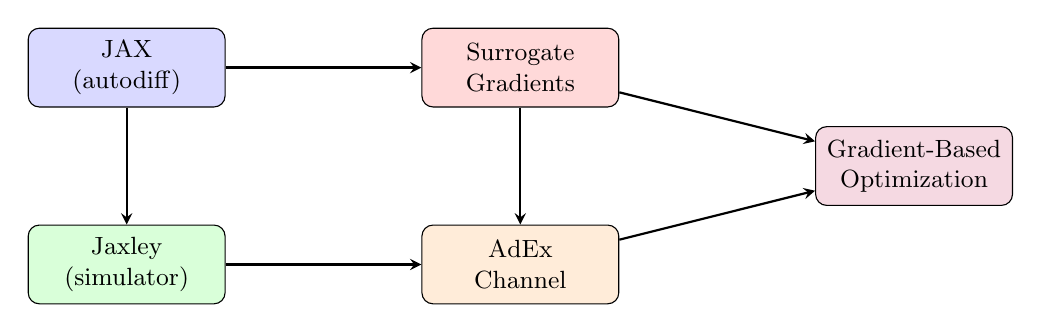
\begin{tikzpicture}[
    box/.style={draw, rounded corners, minimum width=2.5cm, minimum height=1cm, align=center, font=\small},
    arrow/.style={->, thick, >=stealth}
]
    \node[box, fill=blue!15] (jax) at (0,2.5) {JAX\\(autodiff)};
    \node[box, fill=green!15] (jaxley) at (0,0) {Jaxley\\(simulator)};
    \node[box, fill=orange!15] (adex) at (5,0) {AdEx\\Channel};
    \node[box, fill=red!15] (surr) at (5,2.5) {Surrogate\\Gradients};
    \node[box, fill=purple!15] (opt) at (10,1.25) {Gradient-Based\\Optimization};

    \draw[arrow] (jax) -- (jaxley);
    \draw[arrow] (jaxley) -- (adex);
    \draw[arrow] (surr) -- (adex);
    \draw[arrow] (jax) -- (surr);
    \draw[arrow] (adex) -- (opt);
    \draw[arrow] (surr) -- (opt);
\end{tikzpicture}
\end{center}

\vspace{0.5cm}
\textbf{Continuous reset formulation:}
\[
V_{\text{new}} = s \cdot V_r + (1 - s) \cdot V, \quad s = \tilde{H}(V - V_{\text{th}})
\]
\end{frame}

%% ============================================================
%% SLIDE 7: Verification
%% ============================================================
\begin{frame}{Implementation Verification}
\begin{center}

\includegraphics[width=\textwidth]{figures/adex_comparison_combined.pdf}
\end{center}
\vspace{-0.3cm}
\small Comparison against Brian2 reference simulator across three parameter sets
\end{frame}

%% ============================================================
%% SLIDE 8: Research Question
%% ============================================================
\begin{frame}{Research Question}
\begin{center}
\Large
\textbf{What loss function enables successful\\parameter fitting?}
\end{center}

\vspace{1cm}
\begin{columns}[T]
\begin{column}{0.45\textwidth}
\centering
\textbf{MSE Loss}\\[0.3cm]
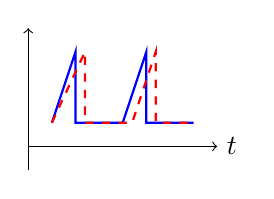
\begin{tikzpicture}[scale=0.6]
    \draw[->] (0,0) -- (4,0) node[right] {$t$};
    \draw[->] (0,-0.5) -- (0,2.5);
    \draw[blue, thick] (0.5,0.5) -- (1,2) -- (1,0.5) -- (2,0.5) -- (2.5,2) -- (2.5,0.5) -- (3.5,0.5);
    \draw[red, thick, dashed] (0.5,0.5) -- (1.2,2) -- (1.2,0.5) -- (2.2,0.5) -- (2.7,2) -- (2.7,0.5) -- (3.5,0.5);
\end{tikzpicture}\\
\small Sample-by-sample
\end{column}
\begin{column}{0.45\textwidth}
\centering
\textbf{Feature-Based}\\[0.3cm]
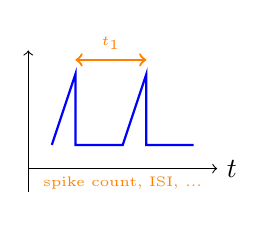
\begin{tikzpicture}[scale=0.6]
    \draw[->] (0,0) -- (4,0) node[right] {$t$};
    \draw[->] (0,-0.5) -- (0,2.5);
    \draw[blue, thick] (0.5,0.5) -- (1,2) -- (1,0.5) -- (2,0.5) -- (2.5,2) -- (2.5,0.5) -- (3.5,0.5);
    \draw[<->, orange, thick] (1,2.3) -- node[above, font=\tiny] {$t_1$} (2.5,2.3);
    \node[orange, font=\tiny] at (2,-0.3) {spike count, ISI, ...};
\end{tikzpicture}\\
\small Firing features
\end{column}
\end{columns}
\end{frame}

%% ============================================================
%% SLIDE 9: MSE Problem
%% ============================================================
\begin{frame}{MSE Loss: Why It Fails}
\begin{center}
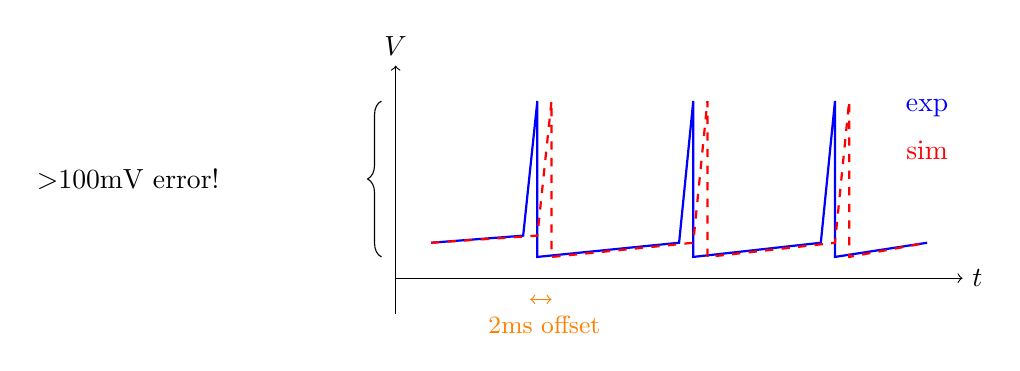
\begin{tikzpicture}[scale=0.9]
    % Two traces with slight offset
    \draw[->] (0,0) -- (8,0) node[right] {$t$};
    \draw[->] (0,-0.5) -- (0,3) node[above] {$V$};

    % Experimental trace
    \draw[blue, thick] (0.5,0.5) -- (1.8,0.6) -- (2,2.5) -- (2,0.3) -- (4,0.5) -- (4.2,2.5) -- (4.2,0.3) -- (6,0.5) -- (6.2,2.5) -- (6.2,0.3) -- (7.5,0.5);

    % Simulated trace (offset)
    \draw[red, thick, dashed] (0.5,0.5) -- (2,0.6) -- (2.2,2.5) -- (2.2,0.3) -- (4.2,0.5) -- (4.4,2.5) -- (4.4,0.3) -- (6.2,0.5) -- (6.4,2.5) -- (6.4,0.3) -- (7.5,0.5);

    % Highlight mismatch
    \draw[<->, orange, thin] (1.9,-0.3) -- (2.2,-0.3);
    \node[orange, below] at (2.1,-0.4) {\small 2ms offset};

    % Error annotation
    \draw[decorate, decoration={brace, amplitude=5pt}] (-0.2,0.3) -- (-0.2,2.5);
    \node[right] at (-5.2,1.4) {\alert{$>$100mV error!}};

    \node[blue] at (7.5,2.4) {exp};
    \node[red] at (7.5,1.8) {sim};
\end{tikzpicture}
\end{center}

\begin{itemize}
    \item Small timing offset $\Rightarrow$ huge MSE
    \item Optimizer learns to \alert{suppress spikes} to minimize loss
\end{itemize}
\end{frame}

%% ============================================================
%% SLIDE 10: MSE Results
%% ============================================================
\begin{frame}{MSE Training Results}
\begin{center}

\includegraphics[width=\textwidth]{figures/mse_training_results.pdf}
\end{center}
\vspace{-0.3cm}
Model converges to \alert{non-spiking} solution to minimize subthreshold error
\end{frame}

%% ============================================================
%% SLIDE 11: Feature-Based Loss
%% ============================================================
\begin{frame}{Feature-Based Loss (Guarino et al.)}
\begin{center}
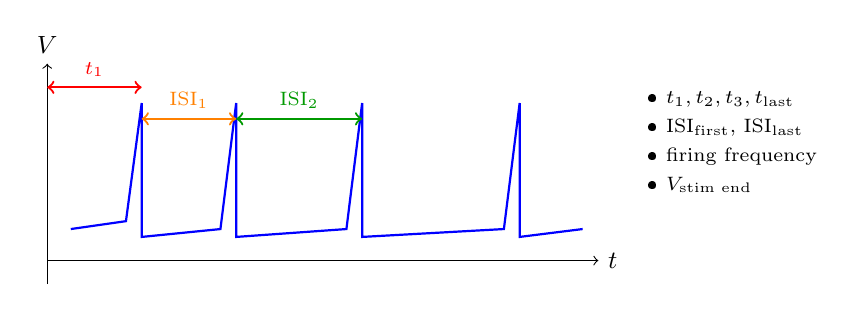
\begin{tikzpicture}[font=\small]
    % Voltage trace
    \draw[->] (0,0) -- (7,0) node[right] {$t$};
    \draw[->] (0,-0.3) -- (0,2.5) node[above] {$V$};

    % Spikes
    \draw[blue, thick]
        (0.3,0.4) -- (1,0.5) -- (1.2,2) -- (1.2,0.3)
        -- (2.2,0.4) -- (2.4,2) -- (2.4,0.3)
        -- (3.8,0.4) -- (4,2) -- (4,0.3)
        -- (5.8,0.4) -- (6,2) -- (6,0.3) -- (6.8,0.4);

    % Feature annotations
    \draw[<->, red, thick] (0,2.2) -- node[above, font=\scriptsize] {$t_1$} (1.2,2.2);
    \draw[<->, orange, thick] (1.2,1.8) -- node[above, font=\scriptsize] {ISI$_1$} (2.4,1.8);
    \draw[<->, green!60!black, thick] (2.4,1.8) -- node[above, font=\scriptsize] {ISI$_2$} (4,1.8);

    % Feature list
    \node[right, align=left, font=\scriptsize] at (7.5,1.5) {
        \textbullet\ $t_1, t_2, t_3, t_{\text{last}}$\\[.3em]
        \textbullet\ ISI$_{\text{first}}$, ISI$_{\text{last}}$\\[.3em]
        \textbullet\ firing frequency\\[.3em]
        \textbullet\ $V_{\text{stim end}}$
    };
\end{tikzpicture}
\end{center}

\vspace{0.3cm}
\[
\mathcal{L}_{\text{feature}} = \sum_i w_i \cdot \frac{|f_i^{\text{sim}} - f_i^{\text{exp}}|}{|f_i^{\text{exp}}| + \epsilon}
\]

Captures \textbf{what matters}: firing pattern, not exact voltage trace
\end{frame}

%% ============================================================
%% SLIDE 12: Feature-Based Results
%% ============================================================
\begin{frame}{Feature-Based Training Results}
\begin{center}

\includegraphics[width=\textwidth]{figures/guarino_training_results.pdf}
\end{center}
\vspace{-0.3cm}
Better captures firing patterns, but non-monotonic loss indicates \alert{non-convex} landscape
\end{frame}

%% ============================================================
%% SLIDE 13: Evaluation
%% ============================================================
\begin{frame}{Evaluation: Coincidence Factor $\Gamma$}
\begin{center}

\includegraphics[width=\textwidth]{figures/coincidence_evaluation.pdf}
\end{center}
\vspace{-0.2cm}
\begin{center}
Both approaches: $\Gamma \approx 0$ (chance level)\\
\small Reference: well-fitted AdEx achieves $\Gamma \approx 0.82$
\end{center}
\end{frame}

%% ============================================================
%% SLIDE 14: Conclusion
%% ============================================================
\begin{frame}{Key Findings}
\begin{columns}[T]
\begin{column}{0.5\textwidth}
\textbf{What worked:}
\begin{itemize}
    \item[$\checkmark$] AdEx implementation in Jaxley
    \item[$\checkmark$] Surrogate gradients enable differentiation
    \item[$\checkmark$] Feature-based loss captures firing patterns
\end{itemize}
\end{column}
\begin{column}{0.5\textwidth}
\textbf{What didn't:}
\begin{itemize}
    \item[$\times$] MSE fails completely
    \item[$\times$] Spike timing precision ($\Gamma \approx 0$)
    \item[$\times$] Non-convex optimization landscape
\end{itemize}
\end{column}
\end{columns}

\vspace{0.8cm}
\begin{block}{Main Insight}
\centering
\textbf{Loss function design} is the critical challenge,\\not the optimization method itself
\end{block}
\end{frame}

%% ============================================================
%% SLIDE 15: Future Work
%% ============================================================
\begin{frame}{Future Work}
\begin{center}
\begin{itemize}
  \item Better loss function design (spike-timing aware)
  \item Multiple neuron types and recordings
  \item Systematic surrogate gradient comparison
  \item Benchmark against genetic algorithms (runtime and performance)
\end{itemize}
\end{center}
\end{frame}


%% ============================================================
%% APPENDIX
%% ============================================================
\appendix
\section{Appendix}
\insertsectionpage

%% A1: AdEx Equations Detail
\begin{frame}{A1: AdEx Model Parameters}
\begin{table}
\centering
\small
\begin{tabular}{llll}
\toprule
\textbf{Parameter} & \textbf{Symbol} & \textbf{Default} & \textbf{Unit} \\
\midrule
Membrane capacitance & $C$ & 200 & pF \\
Leak conductance & $g_L$ & 10 & nS \\
Leak reversal & $E_L$ & -70 & mV \\
Threshold potential & $V_T$ & -50 & mV \\
Slope factor & $\Delta_T$ & 2 & mV \\
Reset potential & $V_r$ & -58 & mV \\
Detection threshold & $v_{\text{th}}$ & 0 & mV \\
Adaptation time constant & $\tau_w$ & 30 & ms \\
Subthreshold adaptation & $a$ & 2 & nS \\
Spike-triggered adaptation & $b$ & 0 & pA \\
\bottomrule
\end{tabular}
\end{table}
\end{frame}

%% A2: Surrogate Gradient Math
\begin{frame}{A2: Surrogate Gradient Functions}
\textbf{Sigmoid surrogate:}
\[
\frac{\partial \tilde{H}}{\partial x} = \beta \cdot \sigma(\beta x) \cdot (1 - \sigma(\beta x))
\]

\textbf{Exponential surrogate:}
\[
\frac{\partial \tilde{H}}{\partial x} = \beta \cdot \exp(-\beta |x|)
\]

\textbf{SuperSpike surrogate:}
\[
\frac{\partial \tilde{H}}{\partial x} = \frac{1}{(\beta |x| + 1)^2}
\]

\vspace{0.5cm}
$\beta$ controls sharpness; $x = V - V_{\text{th}}$
\end{frame}

%% A3: Hyperparameters
\begin{frame}{A3: Training Hyperparameters}
\begin{table}
\centering
\small
\begin{tabular}{lcc}
\toprule
\textbf{Parameter} & \textbf{MSE} & \textbf{Guarino} \\
\midrule
Optimizer & Adam & Adam \\
Learning rate & 0.1 & 0.1 \\
Gradient clipping & 2.0 & 2.0 \\
Epochs & 500 & 500 \\
Surrogate type & sigmoid & sigmoid \\
Surrogate slope ($\beta$) & 25.0 & 25.0 \\
\bottomrule
\end{tabular}
\end{table}

\vspace{0.5cm}
\small Note: Hyperparameters not extensively tuned
\end{frame}

%% A4: Dataset
\begin{frame}{A4: Dataset}
\textbf{Source:} Johansson \& Silberberg (2020)

\vspace{0.5cm}
\textbf{Recording type:} Intracellular, current-clamp

\vspace{0.5cm}
\textbf{Neuron type:} Striatal projection neurons (SPN)

\vspace{0.5cm}
\textbf{Limitation:} Single trace used (time constraints)

\vspace{0.5cm}
\textbf{Files:}
\begin{itemize}
    \item Voltage: \texttt{ECBL\_IDthresh\_ch5\_553.dat}
    \item Current: \texttt{ECBL\_IDthresh\_ch4\_553.dat}
\end{itemize}
\end{frame}

%% A5: Spike Timing Table
\begin{frame}{A5: Implementation Verification Results}
\begin{table}
\centering
\begin{tabular}{lccc}
\toprule
 & Tonic & Adaptation & Original \\
\midrule
Spike count & 52 & 10 & 64 \\
Max timing diff.\ (ms) & 0.54 & 0.58 & 0.82 \\
Mean timing diff.\ (ms) & 0.28 & 0.27 & 0.42 \\
\bottomrule
\end{tabular}
\end{table}

\vspace{0.5cm}
Comparison between Jaxley and Brian2 implementations

\vspace{0.3cm}
$\Rightarrow$ Identical spike counts, timing differences $<1$ms
\end{frame}

%% A6: Surrogate Types
\begin{frame}{A6: Why Sigmoid Surrogate?}
\begin{center}

\includegraphics[width=0.8\textwidth]{figures/surrogate_gradients_comparison.pdf}
\end{center}

\begin{itemize}
    \item All three surrogates implemented
    \item Sigmoid commonly used in SNN literature
    \item \alert{Systematic comparison not yet performed}
\end{itemize}
\end{frame}

%% A7: Coincidence Factor Formula
\begin{frame}{A7: Coincidence Factor $\Gamma$}
\[
\Gamma = \frac{N_{\text{coinc}} - \langle N_{\text{coinc}} \rangle}{0.5(N_{\text{data}} + N_{\text{model}})} \cdot \frac{1}{1 - 2f\Delta}
\]

\vspace{0.5cm}
\begin{itemize}
    \item $N_{\text{coinc}}$: coincidences within $\pm\Delta$ (2ms)
    \item $f$: model firing rate
    \item $\Gamma = 1$: perfect prediction
    \item $\Gamma = 0$: chance level
    \item $\Gamma < 0$: worse than chance
\end{itemize}

\vspace{0.5cm}
Reference (Jolivet et al.): well-fitted AdEx achieves $\Gamma \approx 0.82$
\end{frame}

\end{document}
